% ============================================================================
% Informe: Vision Transformer implementado desde cero en CUDA puro.
%
% Compilar con:   tectonic informe/informe.tex
%
% Las figuras (figs/) y las tablas (tables/) las genera automaticamente
%     python3 scripts/make_report_assets.py
% a partir de los CSV de results/. NO editar las tablas a mano: se sobrescriben
% en cada reentrenamiento.
% ============================================================================
\documentclass[11pt,a4paper]{article}

% tectonic usa el motor XeTeX. Aqui va fontspec y NO inputenc/fontenc[T1]:
% comprobado que con [T1]{fontenc} los signos de apertura salen mal ("¿" se
% imprime como "£" y "¡" como "ą"), porque el codepoint Unicode se entrega tal
% cual a una fuente de 8 bits. fontspec usa Latin Modern en OpenType, que
% tectonic descarga solo, y resuelve todos los caracteres del espanol.
\usepackage{fontspec}
\usepackage[spanish,es-noquoting]{babel}
% babel-spanish titula las tablas como "Cuadro"; se unifica con "Tabla", que es
% como las referencia el texto.
\addto\captionsspanish{\renewcommand{\tablename}{Tabla}}
\usepackage[margin=2.3cm]{geometry}
\usepackage{amsmath}
\usepackage{amssymb}
\usepackage{graphicx}
\usepackage{booktabs}
\usepackage{caption}
\usepackage{url}

\captionsetup{font=small,labelfont=bf}
\setlength{\parskip}{0.35em}
\graphicspath{{figs/}}

% ---------------------------------------------------------------------------
% Cifras clave. Los valores por defecto son marcadores; scripts/make_report_assets.py
% genera tables/kpi.tex, que los reemplaza con los numeros medidos. Gracias a
% \providecommand el documento compila aunque todavia no se hayan corrido los
% experimentos.
% ---------------------------------------------------------------------------
\providecommand{\KpiBestPatch}{\textbf{[pendiente]}}
\providecommand{\KpiBestTokens}{\textbf{[?]}}
\providecommand{\KpiBestAcc}{\textbf{[?]}}
\providecommand{\KpiWorstPatch}{\textbf{[pendiente]}}
\providecommand{\KpiWorstTokens}{\textbf{[?]}}
\providecommand{\KpiWorstAcc}{\textbf{[?]}}
\providecommand{\KpiAccGap}{\textbf{[?]}}
\providecommand{\KpiEpochRatio}{\textbf{[?]}}
\providecommand{\KpiTotalTrainSec}{\textbf{[?]}}
\providecommand{\KpiParams}{\textbf{[?]}}
\providecommand{\KpiSpeedupMax}{\textbf{[?]}}
\providecommand{\KpiSpeedupMin}{\textbf{[?]}}
\providecommand{\KpiSpeedupTokensMax}{\textbf{[?]}}
\providecommand{\KpiSpeedupTokensMin}{\textbf{[?]}}
\providecommand{\KpiSpeedupAtMax}{\textbf{[?]}}
\providecommand{\KpiSpeedupAtMin}{\textbf{[?]}}
\providecommand{\KpiBenchDiff}{\textbf{[?]}}
\providecommand{\KpiEndToEndSpeedup}{\textbf{[?]}}
\providecommand{\KpiPxVSpeedupMin}{\textbf{[?]}}
\providecommand{\KpiPxVSpeedupMax}{\textbf{[?]}}
\providecommand{\KpiPxVSpeedupMinTokens}{\textbf{[?]}}
\providecommand{\KpiQKTSpeedupMin}{\textbf{[?]}}
\providecommand{\KpiQKTSpeedupMax}{\textbf{[?]}}
\providecommand{\KpiQKTSpeedupMinTokens}{\textbf{[?]}}

\IfFileExists{tables/kpi.tex}{% Generado por scripts/make_report_assets.py -- no editar a mano
\renewcommand{\KpiBestPatch}{$14\times14$}
\renewcommand{\KpiBestTokens}{5}
\renewcommand{\KpiBestAcc}{92.30}
\renewcommand{\KpiWorstPatch}{$7\times7$}
\renewcommand{\KpiWorstTokens}{17}
\renewcommand{\KpiWorstAcc}{86.45}
\renewcommand{\KpiAccGap}{5.85}
\renewcommand{\KpiEpochRatio}{7.2}
\renewcommand{\KpiTotalTrainSec}{8}
\renewcommand{\KpiParams}{72\,074}
\renewcommand{\KpiSpeedupMax}{2.08}
\renewcommand{\KpiSpeedupMin}{0.49}
\renewcommand{\KpiSpeedupTokensMax}{50}
\renewcommand{\KpiSpeedupTokensMin}{5}
\renewcommand{\KpiSpeedupAtMax}{2.08}
\renewcommand{\KpiSpeedupAtMin}{0.82}
\renewcommand{\KpiBenchDiff}{0.0}
\renewcommand{\KpiPxVSpeedupMin}{0.49}
\renewcommand{\KpiPxVSpeedupMax}{0.69}
\renewcommand{\KpiPxVSpeedupMinTokens}{17}
\renewcommand{\KpiQKTSpeedupMin}{0.82}
\renewcommand{\KpiQKTSpeedupMax}{2.08}
\renewcommand{\KpiQKTSpeedupMinTokens}{5}
\renewcommand{\KpiEndToEndSpeedup}{1.14}
}{}

\title{\vspace{-1.2cm}Implementación de un Vision Transformer desde cero en CUDA:\\
       impacto del número de parches y de la jerarquía de memoria}
\author{%
  Wilson Ramos Pacco, Jhonatan Usccs Giraldo Bilbao,\\
  Alvaro Sergio Cano Luque, Randú Jean Franco Cerpa García\\[6pt]
  \small Tópicos en Inteligencia Artificial --- Universidad Nacional de San Agustín\\
  \small Repositorio: \url{https://github.com/WilsonRamos/VisTransformer}
}
\date{\today}

\begin{document}
\maketitle
\vspace{-0.8cm}

% ===========================================================================
\section{Contexto}
\label{sec:contexto}

La visión por computadora estuvo dominada durante casi tres décadas por redes
convolucionales \cite{lecun1998gradient}, cuya arquitectura codifica de
fábrica el sesgo inductivo de localidad: un píxel se relaciona
principalmente con sus vecinos inmediatos, aprendida con filtros compartidos
que recorren toda la imagen. Dosovitskiy et al. \cite{dosovitskiy2021image}
mostraron que ese sesgo no es indispensable: un Transformer
\cite{vaswani2017attention} sin ninguna noción incorporada de vecindad
espacial, alimentado con parches de imagen como secuencia de tokens, iguala o
supera a las CNN con datos suficientes. La contrapartida es que el modelo
debe \emph{aprender} desde cero qué parches están relacionados, tarea que la
convolución resuelve por diseño; esta ausencia de sesgo inductivo es
precisamente el mecanismo que la Sección~\ref{sec:exp1} invoca para explicar
por qué, con pocos datos, una secuencia más corta resulta más fácil de
optimizar.

Sobre el tamaño de parche, el propio trabajo de Dosovitskiy et al. reporta un
compromiso contrario al que estudia este trabajo: sobre ImageNet con
preentrenamiento a gran escala, reducir el tamaño de parche (más tokens)
generalmente mejora la precisión, porque el detalle espacial adicional sí
aporta información útil cuando sobran datos e imágenes complejas para
aprovecharlo. Este trabajo se ubica en el extremo opuesto: imágenes de
$28\times28$ muy simples y apenas $5\,000$ ejemplos de entrenamiento. Ese
contraste motiva la lectura de la Sección~\ref{sec:conclusiones}: el
compromiso entre tokens y precisión podría no ser una propiedad fija del
Transformer, sino depender de cuánta información discriminativa hay
realmente para extraer a mayor resolución.

Sobre la jerarquía de memoria, la atención estándar materializa una matriz de
\emph{scores} de $T \times T$, cuyo acceso repetido desde memoria global es
exactamente el cuello de botella que ataca el \emph{tiling} en memoria
compartida, siguiendo el patrón clásico de multiplicación de matrices por
bloques \cite{kirk2016programming}. FlashAttention \cite{dao2022flashattention}
lleva la misma idea más lejos: funde \emph{scores}, softmax y la
multiplicación por $V$ en un único kernel que nunca escribe la matriz
$T\times T$ en memoria global, evitando el problema en vez de solo
mitigarlo. El experimento de memoria de este trabajo
(Sección~\ref{sec:exp2}) estudia la misma palanca a
una escala mucho más pequeña y con los dos kernels sin fusionar, lo que
permite aislar el efecto de cada uno por separado; el hallazgo de que el
beneficio del tiling no es uniforme entre ambos es, en cierto sentido, una
motivación adicional para el enfoque fusionado que usa FlashAttention.

\paragraph{Alcance.} Este trabajo se limita a MNIST, a una arquitectura fija
de dos bloques con $D=64$, a tres tamaños de parche específicos y a una sola
semilla aleatoria por configuración. No evalúa en imágenes naturales de mayor
resolución, no compara contra una implementación fusionada al estilo
FlashAttention, y no repite las corridas para estimar variabilidad (ver
Limitaciones, Sección~\ref{sec:conclusiones}). Dentro de ese alcance, el
objetivo es aislar y explicar dos efectos concretos, no producir un modelo
competitivo con el estado del arte.

% ===========================================================================
\section{Problema}

Los Vision Transformers (ViT) \cite{dosovitskiy2021image} adaptan la arquitectura
Transformer \cite{vaswani2017attention} al dominio visual mediante una idea
sencilla: una imagen se corta en parches cuadrados no solapados, cada parche se
proyecta linealmente a un vector de dimensión $D$, y la secuencia resultante se
procesa con auto-atención exactamente igual que una secuencia de palabras. Esa
decisión de diseño (\emph{cuán grandes son los parches}) gobierna todo lo
demás: fija el número de tokens $T$, y con él tanto el detalle espacial que el
modelo puede representar como el coste computacional, porque la auto-atención
escala como $O(T^2)$.

El problema que aborda este trabajo tiene dos caras. La primera es de
aprendizaje profundo: \textbf{¿qué tamaño de parche conviene para clasificar
dígitos de MNIST \cite{lecun1998gradient}, y cuál es el compromiso real entre
precisión y coste?} La segunda es de programación paralela: los productos
matriciales de la atención son el núcleo computacional del modelo, y su
rendimiento en GPU depende críticamente de cómo se usa la jerarquía de memoria.
\textbf{¿Cuánto se gana al pasar de un kernel que lee todo de memoria global a
uno que reutiliza los datos mediante tiling en memoria compartida, y cómo
depende esa ganancia del número de tokens?}

Ambas preguntas se conectan: cuantos más parches, mayor es la matriz de
atención $T \times T$, y mayor debería ser el beneficio del tiling. Para poder
responderlas con propiedad, el modelo se implementa \textbf{íntegramente con
kernels CUDA propios}, incluido el paso hacia atrás, derivado y programado a
mano capa por capa, sin recurrir a cuDNN ni a cuBLAS. Escribir la
retropropagación a mano no es un capricho: es la única forma de ver
explícitamente cómo circula el gradiente por LayerNorm, por el softmax de la
atención y por cada proyección lineal.

% ===========================================================================
\section{Objetivo}

\paragraph{Objetivo general.} Implementar, entrenar y evaluar un Vision
Transformer completo sobre MNIST usando exclusivamente kernels CUDA escritos
desde cero, y caracterizar experimentalmente el efecto del tamaño de parche y
de la jerarquía de memoria sobre la precisión y el rendimiento.

\paragraph{Objetivos específicos.}
\begin{enumerate}\itemsep2pt
  \item Programar los kernels de propagación hacia adelante y hacia atrás de
        todas las capas del ViT (patch embedding, atención multi-cabeza,
        LayerNorm, MLP con GELU y cabeza de clasificación), con gradientes
        analíticos cerrados y sin diferenciación automática.
  \item Verificar la corrección de la implementación de forma independiente,
        contrastando cada gradiente analítico contra una aproximación numérica
        y la arquitectura completa contra una referencia en PyTorch.
  \item Medir precisión, tiempo de entrenamiento, tiempo de inferencia, uso de
        memoria y número de parámetros para parches de $4\times4$, $7\times7$ y
        $14\times14$, y explicar el compromiso resultante.
  \item Implementar dos versiones del kernel crítico de la atención: una
        basada solo en memoria global y otra con tiling en memoria compartida.
        Medir su tiempo de forma aislada con \texttt{cudaEvent\_t} y cuantificar
        el \emph{speedup} en función del número de tokens.
\end{enumerate}

% ===========================================================================
\section{Metodología}

\subsection{Datos}

Se usan los archivos originales de MNIST en formato IDX. El cargador
(\texttt{src/data\_loader.c}) interpreta la cabecera respetando el orden de
bytes \emph{big-endian} del formato, valida el número mágico
(\texttt{0x00000803} para imágenes, \texttt{0x00000801} para etiquetas),
normaliza los píxeles a $[0,1]$ y deja las imágenes en un bloque contiguo de
\texttt{float} listo para una única transferencia a GPU. Antes de entrenar se
ejecuta un test que dibuja dígitos como \emph{ASCII art} y comprueba que la
media de los píxeles sea $0{,}1307$, el valor conocido de MNIST normalizado; una
media distinta delataría un error de \emph{stride} o de cabecera.

Por presupuesto de tiempo se emplea un subconjunto de $5\,000$ imágenes de
entrenamiento y $2\,000$ de test, configurable con las opciones
\texttt{--train-n} y \texttt{--test-n}.

\subsection{Arquitectura}

El modelo es un ViT reducido, deliberadamente pequeño para que las seis
corridas quepan en el presupuesto de cómputo:

\begin{center}\small
\begin{tabular}{ll}
\toprule
Dimensión de embedding $D$ & 64 \\
Cabezas de atención $H$ & 4 (dimensión por cabeza $D_h = 16$) \\
Bloques Transformer & 2, en configuración \emph{pre-norm} \\
Oculta del MLP & 128 ($2D$) \\
Tokens $T$ & $49{+}1$, $16{+}1$ o $4{+}1$ según el parche \\
Parámetros & $\approx$ \KpiParams \\
\bottomrule
\end{tabular}
\end{center}

La imagen $28\times28$ se divide en parches no solapados; los tres tamaños
elegidos ($4$, $7$ y $14$) son precisamente los divisores de 28 que dan
particiones limpias. Cada parche se aplana a $p^2$ valores y se proyecta a $D$
dimensiones. Se antepone un token \texttt{[CLS]} aprendible, cuya representación
final alimenta la cabeza de clasificación, y se suman \textbf{embeddings
posicionales aprendibles}. Se prefirieron estos a los sinusoidales fijos porque
la longitud de secuencia es constante dentro de cada configuración y muy corta
(entre 5 y 50 posiciones): la tabla aprendible cuesta apenas $T \cdot D$
parámetros y evita justificar una elección arbitraria de frecuencias, pensada
para secuencias de longitud variable.

Cada bloque aplica $x \leftarrow x + \mathrm{Attn}(\mathrm{LN}(x))$ y luego
$x \leftarrow x + \mathrm{MLP}(\mathrm{LN}(x))$. La variante \emph{pre-norm}
\cite{xiong2020layer} normaliza antes de cada submódulo y estabiliza el
entrenamiento sin necesidad de \emph{warmup} del learning rate, algo importante
con un presupuesto de solo 15 épocas. La activación del MLP es GELU
\cite{hendrycks2016gaussian} en su aproximación con tangente hiperbólica.

\subsection{Retropropagación analítica}

Todo el paso hacia atrás está derivado a mano. Para una capa lineal
$Y = XW + b$ con $X \in \mathbb{R}^{M\times K}$ y $W \in \mathbb{R}^{K\times N}$
se usan las tres identidades
\begin{equation}
\frac{\partial \mathcal{L}}{\partial X} = \frac{\partial \mathcal{L}}{\partial Y} W^{T},
\qquad
\frac{\partial \mathcal{L}}{\partial W} = X^{T} \frac{\partial \mathcal{L}}{\partial Y},
\qquad
\frac{\partial \mathcal{L}}{\partial b_n} = \sum_{m} \frac{\partial \mathcal{L}}{\partial Y_{mn}} ,
\end{equation}
que corresponden exactamente a los tres kernels \texttt{gemm\_nt},
\texttt{gemm\_tn} y \texttt{bias\_backward}.

Para LayerNorm \cite{ba2016layer}, con $\hat{x} = (x-\mu)/\sigma$, $r = 1/\sigma$ y
$g$ el parámetro de escala, los términos que pasan por $\mu$ y por $\sigma$ se
agrupan hasta llegar a la forma compacta que implementa el kernel:
\begin{equation}
\frac{\partial \mathcal{L}}{\partial x_j}
  = r\left(\delta_j - \overline{\delta} - \hat{x}_j\,\overline{\delta\hat{x}}\right),
  \qquad \delta_j = \frac{\partial \mathcal{L}}{\partial y_j}\, g_j ,
\end{equation}
donde las barras denotan promedios sobre la dimensión normalizada. Es decir,
dos productos escalares por fila, resueltos con reducciones en memoria
compartida.

Para el softmax por filas de la atención, con $p = \mathrm{softmax}(s)$, la
jacobiana $\partial p_i/\partial s_j = p_i(\delta_{ij}-p_j)$ colapsa en
\begin{equation}
\frac{\partial \mathcal{L}}{\partial s_j}
  = p_j\left(\frac{\partial \mathcal{L}}{\partial p_j}
    - \sum_k p_k \frac{\partial \mathcal{L}}{\partial p_k}\right).
\end{equation}
Finalmente, softmax y entropía cruzada se derivan de forma conjunta, lo que
cancela términos y deja simplemente
$\partial \mathcal{L}/\partial \text{logits} = (p - \mathbf{1}_y)/B$, una
expresión mucho más estable numéricamente que encadenar ambas por separado.

El optimizador es AdamW \cite{loshchilov2019decoupled} implementado como un
único kernel elemental sobre todo el bloque contiguo de parámetros. Se eligió
Adam sobre SGD porque los Transformers son notoriamente sensibles al learning
rate con SGD y con 15 épocas no hay margen para ajustarlo.

\subsection{Diseño de los kernels}
\label{sec:diseno}

Los productos matriciales usan bloques de $16\times16 = 256$ hilos, múltiplo del
tamaño de warp y con buena ocupación en una T4 \cite{nvidia2024cuda}. Cada bloque
calcula un tile de $16\times16$ de la salida; el recorrido de la dimensión
contraída se hace por tiles, trayendo cooperativamente un fragmento de cada
operando a memoria compartida \cite{kirk2016programming}. Los arreglos
compartidos llevan una columna de relleno (\texttt{[16][17]}) para romper la
alineación con los 32 bancos de memoria compartida y evitar conflictos al leer
columnas. Los kernels elemento a elemento (GELU, residuales, Adam) usan bloques
unidimensionales de 256 hilos con un hilo por elemento y accesos perfectamente
coalescidos, ya que están limitados por ancho de banda y no por cómputo. Cada
lanzamiento va seguido de \texttt{cudaGetLastError()}; compilando con
\texttt{-DVIT\_DEBUG} se añade además \texttt{cudaDeviceSynchronize()} para
localizar errores asíncronos de ejecución.

Un detalle relevante para interpretar el experimento de memoria de la
Sección~\ref{sec:exp2}: el kernel de $QK^{T}$ y el de $P\cdot V$ tienen la
dimensión contraída $K$ en lugares distintos. En $QK^{T}$, $K = D_h = 16$
(exactamente el ancho de un tile), así que el bucle de tiling ejecuta
\emph{una sola iteración}. En $P\cdot V$, en cambio, $K = T$ (hasta 50), así
que ese mismo bucle necesita hasta $\lceil 50/16 \rceil = 4$ iteraciones, cada
una con dos barreras \texttt{\_\_syncthreads()}. Esta diferencia estructural
resulta decisiva para explicar por qué el tiling beneficia a un kernel y
perjudica al otro.

\subsection{Entorno y protocolo de medición}

El entrenamiento se ejecuta en Google Colab con GPU NVIDIA T4 (arquitectura
Turing, \texttt{sm\_75}), compilando con \texttt{nvcc -O3}. Los tiempos se miden
con \texttt{cudaEvent\_t}, que registra tiempo de GPU y no de CPU, lo correcto
para kernels asíncronos. El microbenchmark del experimento 2 descarta
iteraciones de calentamiento (la primera invocación incluye la carga del módulo
y la compilación JIT del PTX), promedia sobre 200 repeticiones dentro de una
única ventana de medición para que la latencia de lanzamiento no domine, y
reporta la mediana de 5 ventanas para descartar valores atípicos causados por
otros procesos en la GPU compartida. Para el tiempo por época \emph{extremo a
extremo} con memoria global (Sección~\ref{sec:exp2}), se corrieron solo 3
épocas en vez de 15: ese experimento mide únicamente velocidad, no precisión
final, así que entrenar hasta converger habría gastado presupuesto de GPU sin
aportar nada a la comparación. Por eso la precisión de esas corridas no se
reporta ni se compara con la Tabla~\ref{tab:patch}.

\subsection{Validación de la corrección}

Antes de dar por buena cualquier medición se ejecutan dos controles
independientes. El primero (\texttt{tests/verify\_kernels.cpp}) emula en CPU las
mismas expresiones de índice de los kernels tileados (misma estructura de
bloques, hilos y tiles) y las contrasta contra una implementación ingenua,
incluyendo tamaños que no son múltiplos de 16 para ejercitar las guardas de
frontera; además compara cada gradiente analítico contra su aproximación por
diferencias centradas. El segundo es una réplica exacta de la arquitectura en
PyTorch (\texttt{scripts/vit\_reference.py}) que fija la precisión esperada: si
la versión CUDA queda muy por debajo, el fallo está en los kernels y no en los
hiperparámetros. Sobre el mismo subconjunto y con los mismos hiperparámetros,
esa referencia (ejecutada en CPU/MPS, no en la T4) alcanza $87{,}35$\,\%,
$89{,}05$\,\% y $91{,}30$\,\% de precisión en test para parches de $4\times4$,
$7\times7$ y $14\times14$ respectivamente, de modo que la implementación en
CUDA debe situarse en ese entorno. No se espera una coincidencia exacta,
porque el dispositivo, la inicialización aleatoria y el orden de acumulación en
punto flotante difieren. La misma comprobación sirvió para fijar el learning
rate: con $3\cdot 10^{-4}$ las tres configuraciones quedaban sin converger a
las 15 épocas, con lo que la comparación habría medido velocidad de
convergencia en lugar de calidad del modelo. Por último, el propio
microbenchmark comprueba que las
versiones global y compartida produzcan resultados idénticos antes de
compararlas: un \emph{speedup} sobre un kernel incorrecto no significa nada.

% ===========================================================================
\section{Resultados}

\subsection{Experimento 1: número de parches}
\label{sec:exp1}

% TODO: insertar figura de accuracy vs parches -- la genera automaticamente
% scripts/make_report_assets.py a partir de results/summary_p*_shared.csv
\begin{figure}[h]
  \centering
  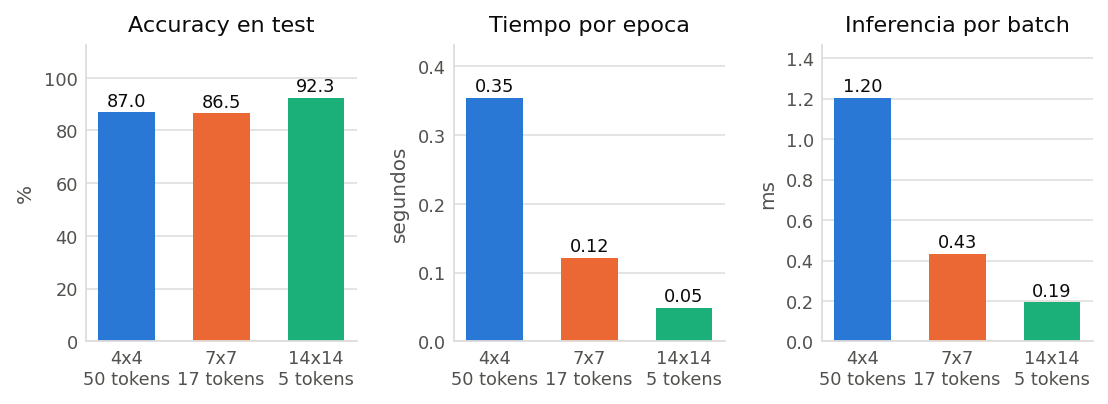
\includegraphics[width=\linewidth]{fig_patch_tradeoff.png}
  \caption{Precisión en test, tiempo por época y tiempo de inferencia por batch
           para los tres tamaños de parche. Menos parches implica menos tokens y,
           por tanto, menos cómputo en la atención.}
  \label{fig:patch}
\end{figure}

% TODO: insertar tabla del experimento 1 -- generada en tables/tab_patch.tex
\begin{table}[h]
  \centering\small
  \caption{Comparación completa por tamaño de parche. Subconjunto de $5\,000$
           imágenes de entrenamiento y $2\,000$ de test, 15 épocas, batch 64,
           AdamW con learning rate $10^{-3}$.}
  \label{tab:patch}
  % Generado por scripts/make_report_assets.py -- no editar a mano
\begin{tabular}{lrrrrrrr}
\toprule
Parche & Tokens & Parametros & Acc. test & Total & s/epoca & Infer. & Mem. GPU \\
 & & & (\%) & (s) & (s) & (ms/batch) & (MiB) \\
\midrule
$4\times4$ & 50 & 72\,074 & 86.95 & 5.3 & 0.35 & 1.20 & 112 \\
$7\times7$ & 17 & 72\,074 & 86.45 & 1.8 & 0.12 & 0.43 & 24 \\
$14\times14$ & 5 & 80\,714 & 92.30 & 0.7 & 0.05 & 0.19 & 6 \\
\bottomrule
\end{tabular}

\end{table}

% ATENCION: el parrafo siguiente describe un hallazgo NO monotonico especifico
% de esta corrida (14x14 gana claro; 4x4 supera a 7x7 por un margen minimo). Si
% se reentrena (mas datos, otra semilla, dataset completo) y el orden cambia,
% hay que revisar a mano tanto los numeros hardcodeados (86,95% para 4x4) como
% la ARGUMENTACION, no solo dejar que kpi.tex actualice las cifras.
La Tabla~\ref{tab:patch} y la Figura~\ref{fig:patch} resumen el experimento. En
\textbf{coste}, el resultado es exactamente el que anticipa la teoría y es
estrictamente monótono en el número de tokens: a más parches, más caro, en los
tres indicadores a la vez (tiempo por época, tiempo de inferencia y memoria de
GPU). El parche $4\times4$ (50 tokens) tarda \KpiEpochRatio{} veces más por
época que el $14\times14$ (5 tokens), consistente con el coste $O(T^2)$ de la
auto-atención.

En \textbf{precisión}, en cambio, el resultado \emph{no} es monótono. La
configuración \KpiBestPatch{} (\KpiBestTokens{} tokens) gana con claridad,
\KpiBestAcc\,\%, muy por encima de las otras dos. Pero entre las dos restantes
el orden se invierte respecto del número de tokens: el parche $4\times4$ (más
tokens, $86{,}95$\,\%) supera ligeramente al $7\times7$ (menos tokens,
\KpiWorstAcc\,\%), una diferencia de apenas medio punto porcentual, dentro
de lo esperable como ruido de una sola corrida con una única semilla aleatoria
(ver Limitaciones). La lectura honesta no es ``menos parches siempre gana'',
sino que \textbf{la configuración extrema de 5 tokens gana por un margen claro
y sistemático} (\KpiAccGap{} puntos sobre la peor de las otras dos, visible ya
desde las primeras épocas en la Figura~\ref{fig:curves}), mientras que la
diferencia entre 17 y 50 tokens no permite concluir nada con un solo experimento
por configuración.

Para el caso claro (por qué 5 tokens gana), la explicación tiene tres
partes. Primero, los dígitos de MNIST son imágenes de $28\times28$ centradas y
de trazo grueso: un parche de $14\times14$ ya cubre un cuadrante completo del
dígito, y la información discriminativa (la topología del trazo) sobrevive a
esa granularidad. Segundo, con 50 tokens el modelo debe aprender 50 embeddings
posicionales a partir de solo $5\,000$ ejemplos, lo que agrava el problema de
optimización sin aportar capacidad útil. Tercero, el ViT carece del sesgo
inductivo de localidad de una convolución: debe \emph{aprender} qué parches son
vecinos, tarea que se vuelve más difícil cuanto más larga es la secuencia. Estos
tres factores explican por qué la secuencia muy corta gana con claridad, pero no
predicen un orden fino entre 17 y 50 tokens; de hecho, los datos tampoco lo
muestran.

% TODO: insertar figura de curvas de perdida y accuracy por epoca
\begin{figure}[h]
  \centering
  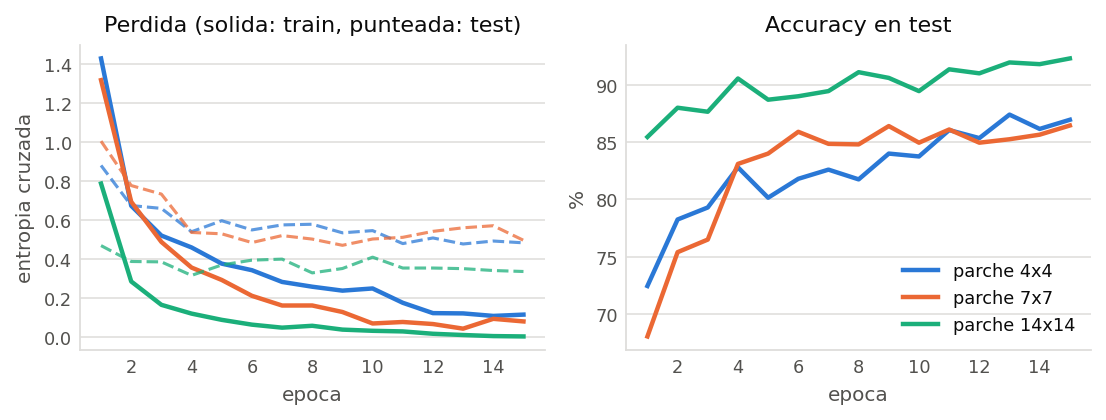
\includegraphics[width=\linewidth]{fig_curves.png}
  \caption{Curvas por época. A la izquierda, entropía cruzada en entrenamiento
           (línea sólida) y en test (punteada); a la derecha, precisión en
           test. El eje $Y$ del panel derecho \textbf{no arranca en 0}: se
           recorta alrededor del rango de datos observado ($68$--$92$\,\%) para
           que las diferencias entre curvas sean visibles, así que las
           distancias verticales entre líneas no deben leerse en proporción.}
  \label{fig:curves}
\end{figure}

Las curvas de la Figura~\ref{fig:curves} muestran además que la configuración de
parche grande no solo termina mejor, sino que \emph{converge antes}: la brecha
entre la pérdida de entrenamiento y la de test indica sobreajuste creciente en
las últimas épocas, esperable con un subconjunto de $5\,000$ imágenes y sin
aumento de datos ni \emph{dropout}.

\subsection{Experimento 2: memoria global frente a memoria compartida}
\label{sec:exp2}

% TODO: insertar figura de tiempo de kernel global vs compartida
\begin{figure}[h]
  \centering
  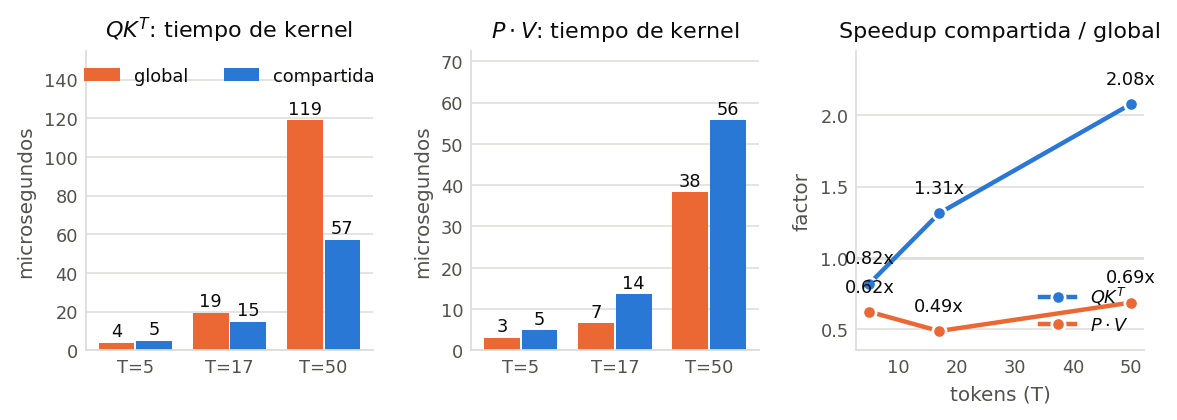
\includegraphics[width=\linewidth]{fig_memory.png}
  \caption{Tiempo de los dos kernels críticos de la atención en sus versiones
           con memoria global y con tiling en memoria compartida, y
           \emph{speedup} resultante en función del número de tokens. En el
           panel derecho, la línea horizontal en $1{,}0\times$ marca la
           ausencia de cambio: por encima, la versión con tiling gana; por
           debajo, pierde frente a la versión con memoria global.}
  \label{fig:memory}
\end{figure}

% TODO: insertar tabla del microbenchmark -- generada en tables/tab_bench.tex
\begin{table}[h]
  \centering\small
  \caption{Microbenchmark aislado de los kernels $QK^{T}$ y $P\cdot V$. Mediana
           de 5 ventanas de 200 repeticiones, con calentamiento descartado.
           Ambas versiones producen resultados bit a bit idénticos (diferencia
           máxima \KpiBenchDiff{} en valor absoluto), así que la diferencia de
           tiempo no se debe a un error de cómputo.}
  \label{tab:bench}
  % Generado por scripts/make_report_assets.py -- no editar a mano
\begin{tabular}{llrrrrr}
\toprule
Kernel & Parche & $T$ & Global & Compartida & Speedup & GFLOP/s \\
 & & & ($\mu$s) & ($\mu$s) & & (compartida) \\
\midrule
$P \cdot V$ & $4\times4$ & 50 & 38.2 & 55.8 & 0.69$\times$ & 367.2 \\
$P \cdot V$ & $7\times7$ & 17 & 6.6 & 13.6 & 0.49$\times$ & 174.4 \\
$P \cdot V$ & $14\times14$ & 5 & 3.0 & 4.8 & 0.62$\times$ & 42.3 \\
$QK^{T}$ & $4\times4$ & 50 & 119.1 & 57.3 & 2.08$\times$ & 357.6 \\
$QK^{T}$ & $7\times7$ & 17 & 19.3 & 14.7 & 1.31$\times$ & 160.7 \\
$QK^{T}$ & $14\times14$ & 5 & 4.0 & 4.9 & 0.82$\times$ & 41.5 \\
\bottomrule
\end{tabular}

\end{table}

El resultado no es el que se suele asumir por defecto, y es el hallazgo más
interesante del trabajo: \textbf{el tiling en memoria compartida no beneficia a
los dos kernels por igual}. $QK^{T}$ sí gana con el tiling, y la ganancia crece
con el número de tokens tal como predice la teoría: a
\KpiSpeedupTokensMax{} tokens el factor es \KpiSpeedupAtMax$\times$, cayendo a
apenas \KpiSpeedupAtMin$\times$ (es decir, la versión con tiling queda
\emph{más lenta}) con solo 5 tokens. $P\cdot V$, en cambio, \textbf{es más
lento con memoria compartida en las tres configuraciones probadas}
(\KpiPxVSpeedupMin$\times$ a \KpiPxVSpeedupMax$\times$, y sin relación monótona
con $T$: el peor caso no ocurre en ningún extremo, sino en
$T=\KpiPxVSpeedupMinTokens$). Ambas versiones producen
resultados idénticos bit a bit (columna \texttt{max\_abs\_diff} de la
Tabla~\ref{tab:bench}), así que la diferencia no es un error de los kernels:
es un efecto real de cómo cada uno usa la memoria.

La explicación está en dónde cae la dimensión contraída $K$ de cada producto,
como se adelantó en la Sección~\ref{sec:diseno}\footnote{Sección
``Diseño de los kernels''.}. En $QK^{T}$, $K = D_h = 16$: el bucle de tiling
ejecuta una única iteración, con una sola ronda de sincronización, y cada
elemento de $Q$ y de $K$ se reutiliza hasta $T$ veces (una por cada fila o
columna de la matriz de \emph{scores} de $T \times T$): la ganancia es real
y crece con $T$ porque crece la reutilización. En $P\cdot V$, $K = T$: para
$T=50$ el bucle necesita $\lceil 50/16 \rceil = 4$ iteraciones, cada una con dos
barreras \texttt{\_\_syncthreads()}, es decir, hasta 8 sincronizaciones de
bloque completo por cada elemento de salida. La reutilización potencial también
existe aquí (cada fila de $P$ se comparte entre los $D_h=16$ hilos que calculan
las columnas de salida), pero el volumen de datos en juego es minúsculo: la
matriz $P$ completa pesa como mucho $50\times50\times4\,\text{B} \approx
10\,\text{KB}$, muy por debajo de la caché L2 de la T4, así que la mayoría de
las lecturas ``redundantes'' de la versión global ya son aciertos de caché casi
tan rápidos como una lectura de memoria compartida. En ese régimen, el costo
fijo de las sincronizaciones adicionales de la versión con tiling pesa más que
el ahorro de ancho de banda que en teoría debería aportar.

Esto también explica el patrón de la Figura~\ref{fig:memory}: la curva de
$QK^{T}$ sube con $T$ porque su única sincronización se amortiza sobre cada vez
más reutilización; la de $P\cdot V$ se mantiene por debajo de $1{,}0\times$
porque el número de sincronizaciones \emph{también} crece con $T$, cancelando
buena parte de la ganancia que el tiling debería aportar. El efecto neto sobre
el entrenamiento completo, donde ambos kernels se ejecutan uno tras otro en
cada paso, es pequeño y a veces se cancela: comparando el tiempo por época de
principio a fin (Tabla~\ref{tab:patch} frente a los mismos experimentos con
memoria global), la versión con tiling resulta más rápida en la configuración
de 5 tokens (hasta \KpiEndToEndSpeedup$\times$) pero prácticamente empatada
en las otras dos (diferencias por debajo del $2$\,\%), porque ahí la pérdida de
$P\cdot V$ absorbe casi toda la ganancia de $QK^{T}$.

% ===========================================================================
\section{Conclusiones}
\label{sec:conclusiones}

\paragraph{Sobre el tamaño de parche.} En MNIST con un presupuesto reducido de
datos, el efecto sobre el \textbf{coste} es limpio y monótono: menos parches es
siempre más barato, con una diferencia de \KpiEpochRatio$\times$ en tiempo por
época entre los extremos, tal como predice el coste $O(T^2)$ de la atención. El
efecto sobre la \textbf{precisión} es más matizado: la configuración de 5 tokens
($14\times14$) gana con claridad (\KpiBestAcc\,\%, entre 5 y 6 puntos por encima
de las otras dos), pero entre 17 y 50 tokens la diferencia es de medio punto
porcentual, indistinguible del ruido con una sola corrida por configuración.
La lección honesta no es que ``menos parches siempre gane'', sino que \textbf{el
extremo de secuencia muy corta gana con claridad}, probablemente porque los
dígitos de MNIST son de trazo grueso y centrados, de modo que la resolución
adicional de más parches no aporta información discriminativa mientras sí agrava
el problema de aprender embeddings posicionales y relaciones espaciales con
pocos datos. Es razonable esperar que el compromiso se invierta en imágenes de
mayor resolución o con objetos descentrados, donde el detalle fino sí sea
necesario.

\paragraph{Sobre la jerarquía de memoria.} Este es el resultado menos esperado
del trabajo: el tiling en memoria compartida \textbf{no benefició a los dos
kernels por igual}. $QK^{T}$ ganó hasta \KpiSpeedupAtMax$\times$, con una
ganancia que crece con el número de tokens como predice la teoría. $P\cdot V$,
en cambio, resultó \emph{más lento} con tiling en las tres configuraciones
probadas (entre \KpiPxVSpeedupMin$\times$ y \KpiPxVSpeedupMax$\times$, sin
relación monótona con $T$). Ambos kernels calculan
exactamente la misma aritmética con exactamente el mismo tamaño de tile, así
que la diferencia no está en un error de implementación sino en la estructura
del problema: $QK^{T}$ tiene su dimensión contraída fija en $D_h=16$ (una sola
iteración de tiling, una sola sincronización), mientras que la de $P\cdot V$ es
el número de tokens $T$ (hasta 4 iteraciones y 8 sincronizaciones para $T=50$).
Con matrices tan pequeñas que caben cómodas en la caché L2 de la GPU, el costo
fijo de esas sincronizaciones adicionales superó el ahorro de ancho de banda que
el tiling debería aportar. La lección práctica, y la más transferible del
trabajo, es que \textbf{el tiling en memoria compartida no es una
optimización universal}: conviene medir cada kernel por separado antes de
asumir que la técnica siempre ayuda, porque su beneficio depende de cuántas
iteraciones necesita el bucle de reducción y de si el problema es lo bastante
grande como para que el tráfico a memoria global, y no la sincronización, sea
el cuello de botella real.

\paragraph{Limitaciones.} Los resultados se obtuvieron con $5\,000$ imágenes de
entrenamiento, 15 épocas y \textbf{una sola semilla aleatoria por
configuración}, lo que impide reportar desviación estándar y hace que
diferencias pequeñas (como la de medio punto entre 17 y 50 tokens) no puedan
distinguirse del ruido de inicialización. Las precisiones absolutas
($\approx 90$\,\%) están muy por debajo del $99$\,\% que alcanzan modelos
convolucionales sobre MNIST completo; la comparación \emph{entre}
configuraciones sigue siendo válida porque todas comparten presupuesto. No se
implementó \emph{dropout} ni aumento de datos, y los kernels usan un tamaño de
tile fijo de $16\times16$ sin ajustar por configuración. El entrenamiento es en
precisión simple, sin aprovechar los \emph{tensor cores} de la T4. Por último,
la explicación del resultado de memoria compartida (Sección~\ref{sec:exp2}) es
mecanística: se apoya en contar iteraciones de tiling y tamaños de matriz,
pero no está confirmada con un perfilador; no se dispuso de \texttt{nsys} o
Nsight Compute en el entorno de Colab usado para separar directamente tiempo de
cómputo, tiempo de memoria y tiempo de sincronización.

\paragraph{Trabajo futuro.} Tres líneas se derivan directamente de las
limitaciones anteriores: repetir cada corrida con varias semillas para
confirmar si la diferencia entre 17 y 50 tokens es señal o ruido; perfilar
los kernels con Nsight Compute para confirmar o refutar la explicación
propuesta para $P\cdot V$; y escalar al conjunto completo de $60\,000$
imágenes para separar el efecto del tamaño de parche del efecto del tamaño de
muestra. Más allá de eso, un tile más pequeño (por ejemplo $8\times8$) podría
ayudar en $T=5$, donde el tile actual excede el tamaño del problema, y una
fusión al estilo FlashAttention (Sección~\ref{sec:contexto}) permitiría
comparar los kernels propios contra cuBLAS con la técnica ya integrada.

% ===========================================================================
{\small
\bibliographystyle{plain}
\bibliography{informe}}

\end{document}
